% !TEX TS-program = lualatex
%\documentclass[handout]{beamer}
\documentclass{beamer}
\input{../common/misomva}
\newcommand{\misoclasstinytitleslide}{Partially based on material by:  Ulrike von Luxburg, \\[-1em] Gary Miller, Doyle \& Schnell, Daniel Spielman}
\newcommand{\misoclassdate}{}
\usetikzlibrary{graphs, shapes.misc, shapes.geometric}

\begin{document}
% Topic-specific title slide

\newcommand{\topictitle}{Spectral Clustering: Examples}

\newcommand{\topicsubtitle}{Understanding and Applications}

\MakeTopicSlide

%%%%%%%%%%%%%%%%%%%%%%%%%%%%%%%%%%%%%%%%%%%%%%%%%%%%%%%%%%%%
\begin{frame}
\frametitle{Spectral Clustering: 1D Example}
 \begin{center}
\onslide<5>{\gcol{Elbow rule/EigenGap heuristic} for number of clusters}\\
\bigskip
\includegraphics<1>[width=\columnwidth]{../img/luxburgh-example-number_1_transparent}%
\includegraphics<2>[width=\columnwidth]{../img/luxburgh-example-number_2_transparent}%
\includegraphics<3>[width=\columnwidth]{../img/luxburgh-example-number_3_transparent}%
\includegraphics<4-5>[width=\columnwidth]{../img/luxburgh-example-number_4_transparent}%
\onslide<5>{\\[-0.5em]{\tiny Source: von Luxburg (2007)}}
\end{center}
\end{frame}
\begin{frame}
\frametitle{Spectral Clustering: Understanding}
%\textbf{Compactness} vs.\@ \emphcol{Connectivity}}
\textbf{Compactness} vs.\@ \emphcol{Connectivity}\\ \medskip
\pause
\resizebox{0.45\columnwidth}{!}{%
\begin{tikzpicture}[scale=2.0]

    % Axes
    \draw[->] (-1.2,-1.6) -- (2.2,-1.6);
    \draw[->] (-1.2,-1.6) -- (-1.2,1.6);
    
    % Labels (Ticks)
    \foreach \x in {-1, -0.5, 0, 0.5, 1, 1.5, 2} \draw (\x,-1.55) -- (\x,-1.65) node[below, font=\tiny] {\x};
    \foreach \y in {-1.5, -1, -0.5, 0, 0.5, 1, 1.5} \draw (-1.15,\y) -- (-1.25,\y) node[left, font=\tiny] {\y};

    % 1. Dark Blue (Top Left) - Slightly vertically elongated
    \foreach \i in {1,\dots,350} {
        \pgfmathsetmacro{\x}{-0.3 + (rand + rand)*0.12}
        \pgfmathsetmacro{\y}{0.8 + (rand + rand)*0.18}
        \node[draw=blue!80!black, circle, inner sep=0.4pt, minimum size=2pt] at (\x, \y) {};
    }
    
    % 2. Orange (Top Right) - Horizontally wide, larger spread
    \foreach \i in {1,\dots,300} {
        \pgfmathsetmacro{\x}{0.6 + (rand + rand)*0.25}
        \pgfmathsetmacro{\y}{0.8 + (rand + rand)*0.12}
        \node[draw=orange, circle, inner sep=0.4pt, minimum size=2pt] at (\x, \y) {};
    }
    
    % 3. Brown (Middle) - Diagonal/Irregular (simulated by correlation)
    % x = rand, y = 0.5*x + rand
    \foreach \i in {1,\dots,300} {
        \pgfmathsetmacro{\u}{(rand + rand)*0.2}
        \pgfmathsetmacro{\v}{(rand + rand)*0.15}
        \pgfmathsetmacro{\x}{0.2 + \u}
        \pgfmathsetmacro{\y}{0.1 + \v - 0.3*\u} % Slight tilt
        \node[draw=brown!70!black, circle, inner sep=0.4pt, minimum size=2pt] at (\x, \y) {};
    }
    
    % 4. Cyan (Bottom Left) - Smaller, tight but dense
    \foreach \i in {1,\dots,250} {
        \pgfmathsetmacro{\x}{-0.5 + (rand + rand)*0.1}
        \pgfmathsetmacro{\y}{-0.5 + (rand + rand)*0.14}
        \node[draw=cyan, circle, inner sep=0.4pt, minimum size=2pt] at (\x, \y) {};
    }
    
    % 5. Green (Bottom Right) - Very flat horizontal ellipse
    \foreach \i in {1,\dots,300} {
        \pgfmathsetmacro{\x}{0.5 + (rand + rand)*0.3}
        \pgfmathsetmacro{\y}{-0.5 + (rand + rand)*0.08}
        \node[draw=green, circle, inner sep=0.4pt, minimum size=2pt] at (\x, \y) {};
    }
    
    % Scattered noise points
    \foreach \i in {1,\dots,40} {
        \pgfmathsetmacro{\x}{-0.8 + rand*0.8}
        \pgfmathsetmacro{\y}{0.0 + rand*1.0}
        \node[draw=blue, circle, inner sep=0.4pt, minimum size=2pt] at (\x, \y) {};
    }
    \foreach \i in {1,\dots,30} {
        \pgfmathsetmacro{\x}{1.2 + rand*0.6}
        \pgfmathsetmacro{\y}{0.5 + rand*0.6}
        \node[draw=orange, circle, inner sep=0.4pt, minimum size=2pt] at (\x, \y) {};
    }

\end{tikzpicture}
}
\resizebox{0.40\columnwidth}{!}{%
\begin{tikzpicture}[scale=1.5]

    % Axes
    \draw[->] (0,0) -- (5.2,0);
    \draw[->] (0,0) -- (0,5.2);
    
    % Labels
    \foreach \x in {0,0.5,\dots,5} \draw (\x,0.05) -- (\x,-0.05) node[below, font=\tiny] {\x};
    \foreach \y in {0,0.5,\dots,5} \draw (0.05,\y) -- (-0.05,\y) node[left, font=\tiny] {\y};

    % Center approx (2.5, 2.5)
    \def\cx{2.5}
    \def\cy{2.5}

    % Inner ring (Blue circles) - Radius approx 0.5
    \foreach \i in {1,\dots,100} {
        \pgfmathsetmacro{\angle}{rand*360}
        \pgfmathsetmacro{\rad}{0.4 + rand*0.15}
        \node[draw=blue, circle, inner sep=0.5pt, minimum size=2pt] at ({\cx + \rad*cos(\angle)}, {\cy + \rad*sin(\angle)}) {};
    }

    % Middle ring (Red crosses) - Radius approx 1.0
    \foreach \i in {1,\dots,150} {
        \pgfmathsetmacro{\angle}{rand*360}
        \pgfmathsetmacro{\rad}{1.0 + rand*0.15}
        % Gap at top? The image has a slight gap or connector at the top
        % Let's just do a full ring for now
        \node[draw=red, cross out, inner sep=0.5pt, minimum size=3pt, rotate=45] at ({\cx + \rad*cos(\angle)}, {\cy + \rad*sin(\angle)}) {};
    }
    % Connector/Bridge at top of red ring extending to green ring
    \foreach \i in {1,\dots,15} {
        \pgfmathsetmacro{\angle}{85 + rand*10}
        % Extend radius from red ring (1.0) towards green ring (2.0)
        \pgfmathsetmacro{\rad}{1.2 + rand*0.6}
        \node[draw=red, cross out, inner sep=0.5pt, minimum size=3pt, rotate=45] at ({\cx + \rad*cos(\angle)}, {\cy + \rad*sin(\angle)}) {};
    }

    % Outer ring (Green triangles) - Radius approx 2.0
    \foreach \i in {1,\dots,250} {
        \pgfmathsetmacro{\angle}{rand*360}
        \pgfmathsetmacro{\rad}{2.0 + rand*0.2}
        \node[draw=green!80!black, regular polygon, regular polygon sides=3, inner sep=0.3pt, minimum size=3pt] at ({\cx + \rad*cos(\angle)}, {\cy + \rad*sin(\angle)}) {};
    }

\end{tikzpicture}
}\\
{\tiny Source: von Luxburg (2007)}
\pause \moves
\questionbox{For which kind of data we can use one vs.\@ the other?}
\pause \moves
\questionbox{Any disadvantages of spectral clustering?}
\end{frame}
\begin{frame}
\frametitle{Spectral Clustering: 1D Example - Histogram}
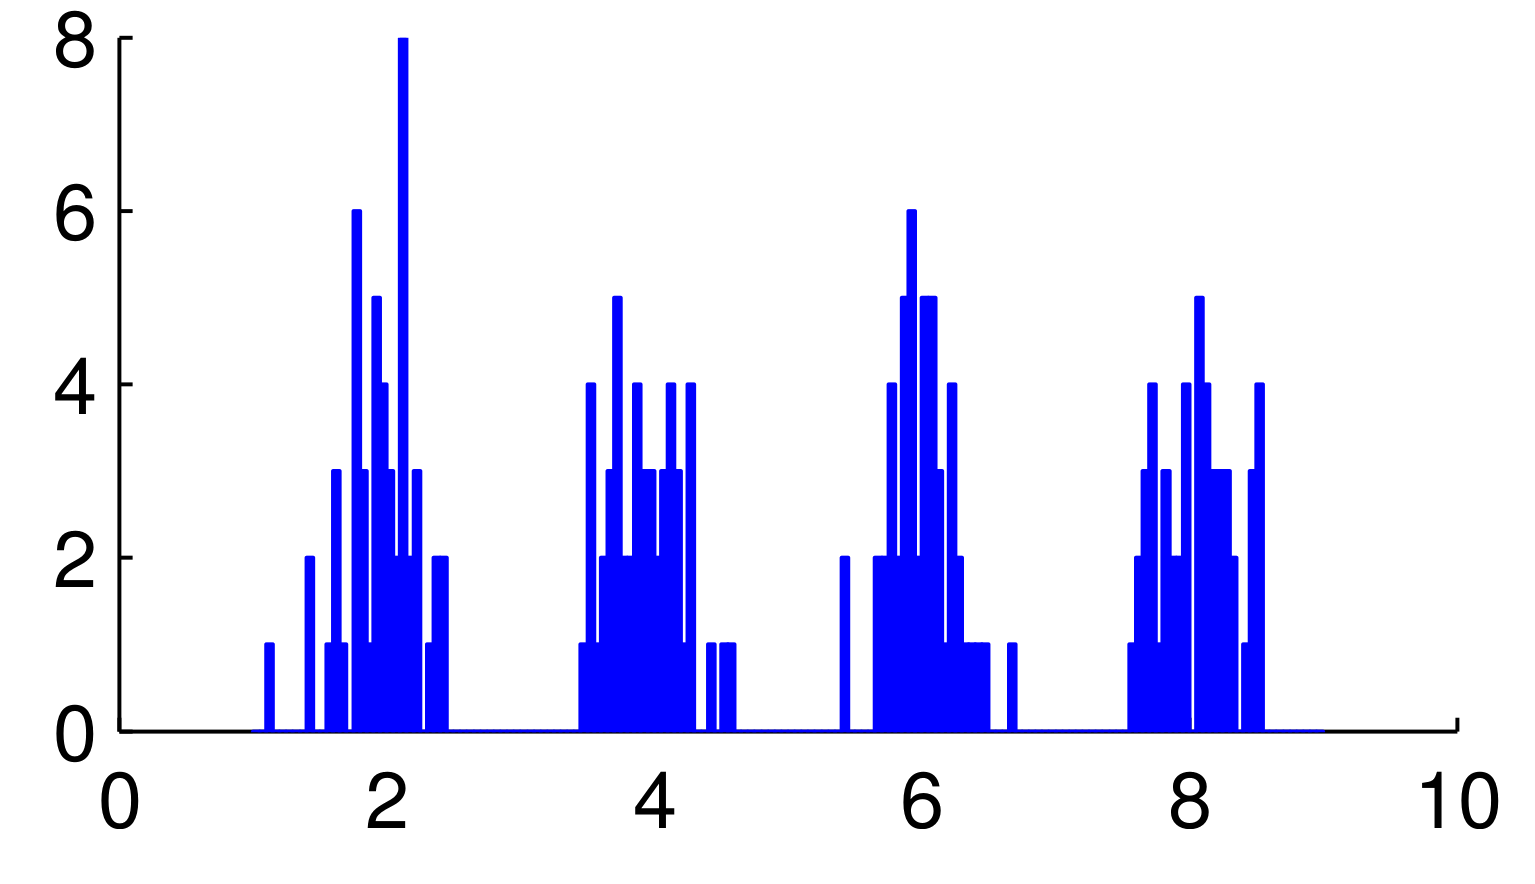
\includegraphics[width=\columnwidth]{../img/luxburgh-example-histogram_transparent}
\\
{\tiny Source: von Luxburg (2007) -- \url{http://www.informatik.uni-hamburg.de/ML/contents/people/luxburg/publications/Luxburg07_tutorial.pdf}}
\end{frame}
\begin{frame}
\frametitle{Spectral Clustering: 1D Example - Eigenvectors}
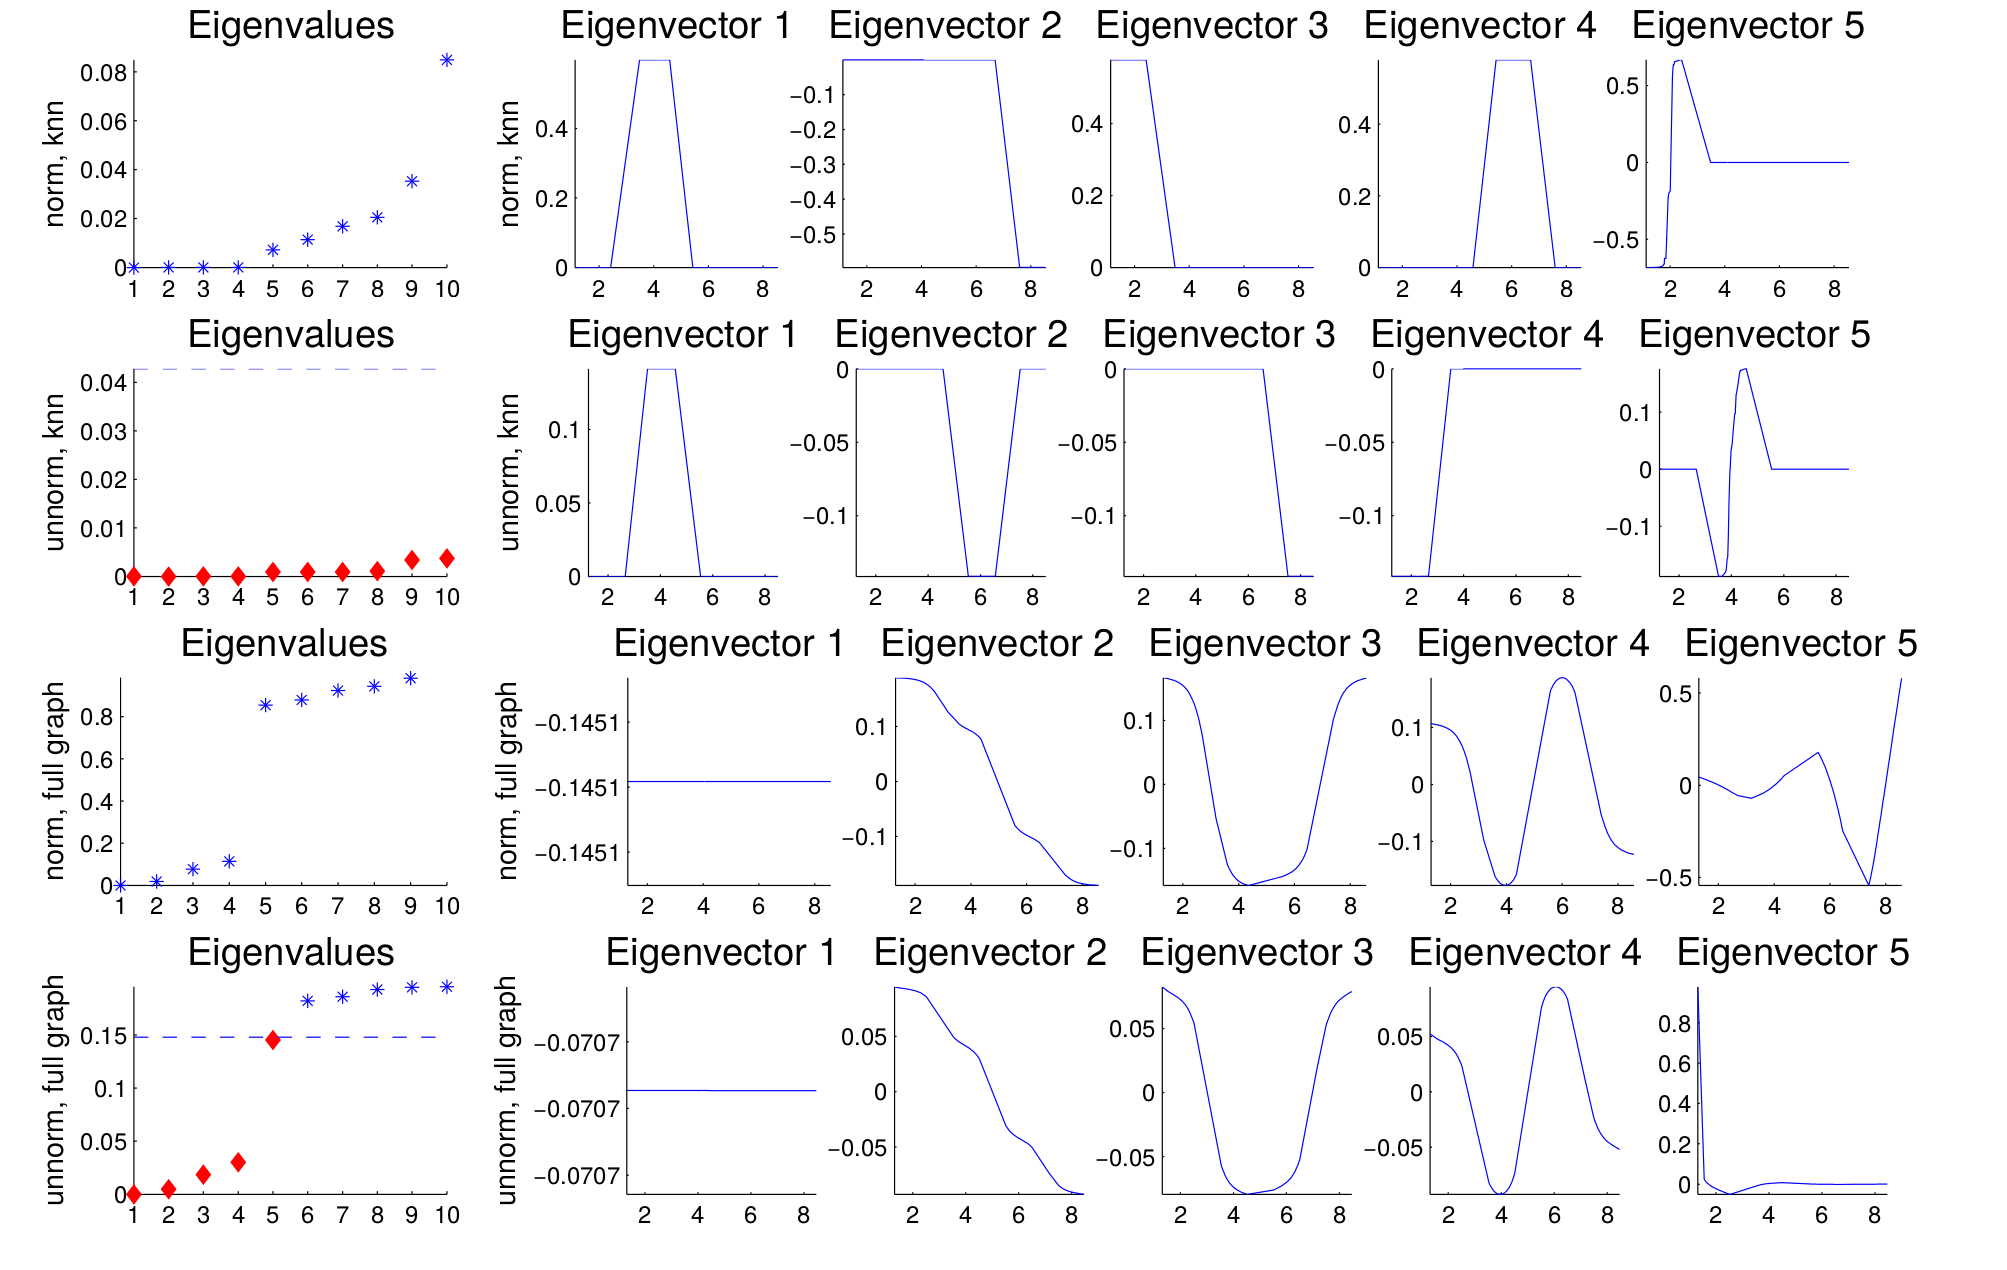
\includegraphics[width=\columnwidth]{../img/luxburgh-example-eigenvectors_transparent}
\\
{\tiny Source: von Luxburg (2007)}
\end{frame}
\begin{frame}
\frametitle{Spectral Clustering: Bibliography}

\begin{itemize}[<+-| alert@+>]\addtolength{\itemsep}{0.5\baselineskip}
\item \href{https://proceedings.mlr.press/v2/meila02a.html}{\textbf{Meila \& Shi (2001)}} -- A random walks view of spectral segmentation\\
{\small \textit{International Conference on Artificial Intelligence and Statistics}}

\item \grcol{$\bL_{\rm sym}$} \href{https://papers.nips.cc/paper/2001/hash/801272ee79cfde7fa5960571fee36b9b-Abstract.html}{\textbf{Ng, Jordan \& Weiss (2001)}} -- On spectral clustering: Analysis and an algorithm\\
{\small \textit{Neural Information Processing Systems (NIPS)}}

\item \grcol{$\bL_{\rm rm}$} \href{https://ieeexplore.ieee.org/document/868688}{\textbf{Shi \& Malik (2000)}} -- Normalized Cuts and Image Segmentation\\
{\small \textit{IEEE Transactions on Pattern Analysis and Machine Intelligence}, 22(8):888--905}

\item \grcol{Things can go wrong with the relaxation:} \href{https://www.sciencedirect.com/science/article/abs/pii/S0024379506003520}{\textbf{Spielman \& Teng (2007)}} -- Spectral partitioning works: Planar graphs and finite element meshes\\
{\small \textit{Linear Algebra and Its Applications}, 421:284--305}
\end{itemize}

\end{frame}


\MakeLastSlide
\end{document}
